            \begin{question}{N.A.}{reconnaissance de courbes}{1}{}
            Parmi les différentes représentations de la figure suivante, laquelle représente une évolution périodique?
            \begin{figure}
            \centering
              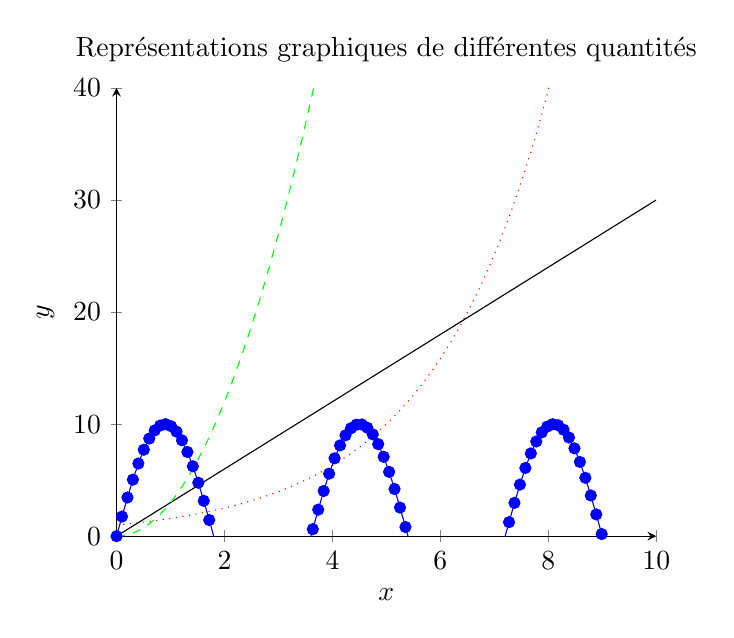
\begin{tikzpicture}
                  \begin{axis}[
                        title = {Représentations graphiques de différentes quantités},
                        axis lines = left,
                        xlabel = $x$,
                        %minor x tick num = 4,
                        ylabel = $y$,
                        ymin=0, ymax=40,
                        /pgf/number format/.cd,%3 lignes dessous, utiliser spacers français au lieu d'anglais.
                        use comma,
                        1000 sep={\,}
                      ]
                      %Below the red curve
                      \addplot [
                        domain=0:10,
                        samples=100,
                        color=red,
                        style=dotted
                        %/pgf/text mark = {+}, %changer le marqueur text
                        %mark=*,
                      ]
                      {10^(0.2*x)};
                      \addplot [
                        domain=0:10,
                        samples=100,
                        color=blue,
                        %/pgf/text mark = {+}, %changer le marqueur text
                        mark=*,
                      ]
                      {10*sin(100*x)};
                      \addplot [
                        domain=0:10,
                        samples=100,
                        color=black,
                        style=solid,
                        %/pgf/text mark = {+}, %changer le marqueur text
                        %mark=o,
                      ]
                      {3*x};
                      \addplot [
                        domain=0:10,
                        samples=100,
                        color=green,
                        style=dashed,
                        %/pgf/text mark = {+}, %changer le marqueur text
                        %mark=triangle,
                      ]
                      {3*x^2};
                  \end{axis}
              \end{tikzpicture}
             \end{figure}
        \end{question}
        \begin{reponses}
            \item[true] La courbe bleue (cercles).
		    \item[false] La courbe rouge (pointillés).
		    \item[false] La courbe noire (pleine).
		    \item[false] La courbe verte (tirets).
		    \end{reponses}
